%-----------------------------------------------------------------------------%
\chapter{\babEmpat}
%\begin{center}
%	\textbf{BAB IV}
%	\par \textbf{ANALISIS SIMULASI SISTEM}
%\end{center}
%-----------------------------------------------------------------------------%

\section{Testing Environment}
Dalam penelitian ini, penulis menggunakan bahasa pemrograman Python untuk membangun dan mengimplementasikan sistem rekomendasi Faculty Supervisor berbasis semantic similarity. Penulis juga menggunakan perangkat keras dan lunak tertentu untuk mengembangkan sistem tersebut. Berikut adalah daftar perangkat keras yang digunakan dalam penelitian ini.
\begin{table}

\centering
\begin{tabular}{|>{\fontsize{11}{14}\selectfont}p{2cm}|>{\fontsize{11}{14}\selectfont}p{5cm}|>{\fontsize{11}{14}\selectfont}p{2cm}|>{\fontsize{11}{14}\selectfont}p{3cm}|}
    \hline
    \textbf{Komponen} & \textbf{Spesifikasi} \\
    \hline
    Processor & Apple M4 Pro (12-core CPU) \\ 
    \hline
    RAM & 24 GB Unified Memory  \\
    \hline
    GPU & Apple M4 Pro Integrated GPU (20-core) + Apple Neural Engine (16-core)  \\
    \hline
    Disk Space & 1 TB SSD \\
    \hline
\end{tabular}
\renewcommand{\arraystretch}{1}
	\caption{Spesifikasi Perangkat Keras}
	\label{table:tab4.1}
\end{table}

Perangkat keras tersebut juga menggunakan beberapa perangkat lunak untuk proses pengembangan sistem rekomendasi Faculty Supervisor. Spesifikasi perangkat lunak yang digunakan adalah sebagai berikut. 

\begin{table}
 \centering
\begin{tabular}{|>{\fontsize{11}{14}\selectfont}p{2cm}|>{\fontsize{11}{14}\selectfont}p{5cm}|>{\fontsize{11}{14}\selectfont}p{2cm}|>{\fontsize{11}{14}\selectfont}p{3cm}|}
    \hline
    \textbf{Komponen} & \textbf{Spesifikasi} \\
    \hline
    Sistem Operasi & macOS Sequoia 15  \\ 
    \hline
    Bahasa Pemrograman  & Python 3.12   \\
    \hline
    Web Framework  & Flask 3.1.0   \\
    \hline
    ORM ; Database  & SQLAlchemy 2.0.49 + SQLite  \\
    \hline
    Embedding Library  & sentence-transformers   \\
    \hline
    Model Kandidat   & BAAI/bge-m3, Qwen/Qwen3-Embedding-0.6B, intfloat/multilingual-e5-large-instruct   \\
    \hline
    Data Processing    & pandas, numpy, openpyxl    \\
    \hline
   IDE    & Visual Studio Code   \\
    \hline
\end{tabular}
\renewcommand{\arraystretch}{1}
	\caption{Spesifikasi Perangkat Lunak}
	\label{table:tab4.2}
\end{table}

\section{Hasil}
\subsection{Evaluasi Model}

Pada tahap ini dilakukan evaluasi terhadap tiga model \textit{embedding} yang menjadi kandidat untuk komponen perhitungan kemiripan semantik. Seluruh model dievaluasi menggunakan \textit{pipeline}, dataset, serta konfigurasi kapasitas yang identik agar perbandingan bersifat adil; satu-satunya variabel yang diubah adalah model \textit{embedding} yang digunakan. Untuk memastikan keterulangan (\textit{reproducibility}), seluruh proses dibuat deterministik sehingga eksekusi berulang menghasilkan keluaran yang identik.

Evaluasi dilakukan terhadap \textbf{168 dari 171 mahasiswa}. Sebanyak 3 mahasiswa dikecualikan karena tidak memiliki nilai \texttt{current\_supervisor\_code} yang valid sebagai \textit{ground truth}.

Pengukuran dilakukan pada dua tingkat yang saling melengkapi:

\begin{itemize}
    \item \textbf{Metrik \textit{retrieval} (sebelum \textit{solver}):} MRR, Hit@1, Hit@5, NDCG@5, NDCG@10, dan rata-rata peringkat (\textit{avg\_rank}). Metrik ini mengukur kualitas pemeringkatan dosen pembimbing sebelum proses alokasi kapasitas dijalankan.
    \item \textbf{Metrik \textit{assignment} (setelah \textit{solver}):} \textit{Assignment Match Rate}. Metrik ini mengukur kesesuaian hasil penugasan akhir terhadap penugasan historis admin.
\end{itemize}

Hasil evaluasi seluruh model kandidat disajikan pada Tabel~\ref{table:tab4.2.1}.

\begin{table}[h]
\centering
\begin{tabular}{|>{\fontsize{9}{12}\selectfont}p{3.2cm}|>{\fontsize{9}{12}\selectfont}p{1.2cm}|>{\fontsize{9}{12}\selectfont}p{1.2cm}|>{\fontsize{9}{12}\selectfont}p{1.2cm}|>{\fontsize{9}{12}\selectfont}p{1.2cm}|>{\fontsize{9}{12}\selectfont}p{1.4cm}|>{\fontsize{9}{12}\selectfont}p{1.4cm}|>{\fontsize{9}{12}\selectfont}p{1.4cm}|}
    \hline
    \textbf{Model} & \textbf{MRR} & \textbf{Hit@1} & \textbf{Hit@5} & \textbf{NDCG@5} & \textbf{NDCG@10} & \textbf{Avg Rank} & \textbf{Match Rate} \\
    \hline
    \textbf{BAAI/bge-m3} (Run 5) & 0,585 & 0,417 & 0,804 & 0,622 & 0,668 & 3,32 & 0,357 \\
    \hline
    \textbf{Qwen/Qwen3-Embedding-0.6B} (Run 6) & 0,474 & 0,298 & 0,708 & 0,505 & 0,576 & 4,20 & 0,357 \\
    \hline
    \textbf{intfloat/multilingual-e5-large-instruct} (Run 9) & 0,469 & 0,304 & 0,649 & 0,483 & 0,563 & 4,60 & 0,381 \\
    \hline
    \textit{Random baseline} & $\sim$0,23 & $\sim$0,07 & $\sim$0,36 & $\sim$0,21 & --- & $\sim$7,5 & --- \\
    \hline
\end{tabular}
\renewcommand{\arraystretch}{1}
    \caption{Perbandingan Metrik Evaluasi Antar Model}
    \label{table:tab4.2.1}
\end{table}

Secara deskriptif, \textbf{BAAI/bge-m3} memperoleh MRR sebesar 0,585 dengan dosen pembimbing sebenarnya berada pada peringkat rata-rata 3,32. \textbf{Qwen/Qwen3-Embedding-0.6B} memperoleh MRR 0,474 dengan rata-rata peringkat 4,20. \textbf{intfloat/multilingual-e5-large-instruct} memperoleh MRR 0,469 dengan rata-rata peringkat 4,60, namun memiliki \textit{Assignment Match Rate} tertinggi sebesar 0,381. Seluruh model berada jauh di atas \textit{random baseline}, yang menunjukkan bahwa pendekatan kemiripan semantik memberikan sinyal pencocokan yang nyata.

Untuk keperluan analisis lebih lanjut, nilai rata-rata skor kemiripan disajikan pada Tabel~\ref{table:tab4.2.2}.

\begin{table}[h]
\centering
\begin{tabular}{|>{\fontsize{11}{14}\selectfont}p{3.5cm}|>{\fontsize{11}{14}\selectfont}p{3cm}|>{\fontsize{11}{14}\selectfont}p{3cm}|>{\fontsize{11}{14}\selectfont}p{2.5cm}|}
    \hline
    \textbf{Model} & \textbf{Avg Similarity @1} & \textbf{Avg True Similarity} & \textbf{Selisih (sebaran)} \\
    \hline
    \textbf{BAAI/bge-m3} (Run 5) & 0,619 & 0,596 & 0,023 \\
    \hline
    \textbf{Qwen/Qwen3-Embedding-0.6B} (Run 6) & 0,692 & 0,624 & 0,068 \\
    \hline
    \textbf{intfloat/multilingual-e5-large-instruct} (Run 9) & 0,871 & 0,857 & 0,014 \\
    \hline
\end{tabular}
\renewcommand{\arraystretch}{1}
    \caption{Rata-rata Skor Kemiripan Antar Model}
    \label{table:tab4.2.2}
\end{table}

\subsection{Hasil Analisis Model dan Pemilihan Model Akhir}

Berdasarkan hasil pada Tabel~\ref{table:tab4.2.1}, \textbf{BAAI/bge-m3} unggul pada seluruh metrik \textit{retrieval}: MRR, Hit@1, Hit@5, NDCG@5, NDCG@10, dan rata-rata peringkat terbaik (3,32). Keunggulan ini konsisten di setiap metrik, bukan hanya pada satu indikator, sehingga menunjukkan kualitas pemeringkatan yang lebih baik secara menyeluruh.

Temuan yang menarik muncul pada \textbf{intfloat/multilingual-e5-large-instruct}. Model ini memiliki \textit{Assignment Match Rate} tertinggi (0,381), namun justru memperoleh metrik \textit{retrieval} terburuk di antara seluruh kandidat. Anomali ini dapat dijelaskan melalui Tabel~\ref{table:tab4.2.2}: \textbf{intfloat/multilingual-e5-large-instruct} menghasilkan skor kemiripan yang sangat tinggi namun nyaris seragam (rata-rata skor peringkat-1 sebesar 0,871 dan skor dosen sebenarnya 0,857, dengan sebaran hanya 0,014). Artinya, model ini menilai hampir seluruh pasangan mahasiswa--dosen sebagai ``sangat mirip'' sehingga kehilangan kemampuan untuk membedakan satu dosen dari dosen lainnya. Tingginya \textit{match rate} pada model ini bukan berasal dari kualitas pemeringkatan, melainkan merupakan efek dari proses alokasi berbasis kapasitas yang kebetulan sejalan dengan beberapa penugasan historis pada skor yang nyaris datar.

Temuan ini menegaskan prinsip penting dalam pemilihan model: \textbf{sebuah sistem rekomendasi dinilai dari kualitas pemeringkatannya} --- yaitu kemampuan menempatkan dosen yang tepat pada posisi teratas --- sehingga metrik \textit{retrieval} menjadi acuan utama. \textit{Assignment Match Rate} merupakan metrik hasil akhir yang bersifat melengkapi, namun apabila digunakan sendirian dapat menyesatkan, sebagaimana ditunjukkan oleh kasus \textbf{intfloat/multilingual-e5-large-instruct}.

Dengan pertimbangan tersebut, \textbf{BAAI/bge-m3} dipilih sebagai model akhir yang digunakan dalam sistem. Pemilihan ini didasarkan pada keunggulan menyeluruh pada metrik \textit{retrieval}, yang merupakan indikator paling representatif terhadap tujuan utama sistem, yaitu memberikan rekomendasi dosen pembimbing yang relevan. Selain itu, hasil model ini telah diverifikasi bersifat deterministik dan dapat direproduksi secara identik pada eksekusi berulang, sehingga angka yang dilaporkan dapat dipertanggungjawabkan.

\subsection{Aplikasi Web}

Sistem rekomendasi mahasiswa ini diimplementasikan dalam bentuk aplikasi berbasis web dengan antarmuka yang fungsional. Aplikasi ini dirancang untuk memfasilitasi Enrichment Program Coordinator dalam melakukan pemetaan (mapping) antara mahasiswa peserta program enrichment dengan faculty supervisor terkait.   

\subsubsection{Login Page}

\begin{figure}
    \begin{center}
        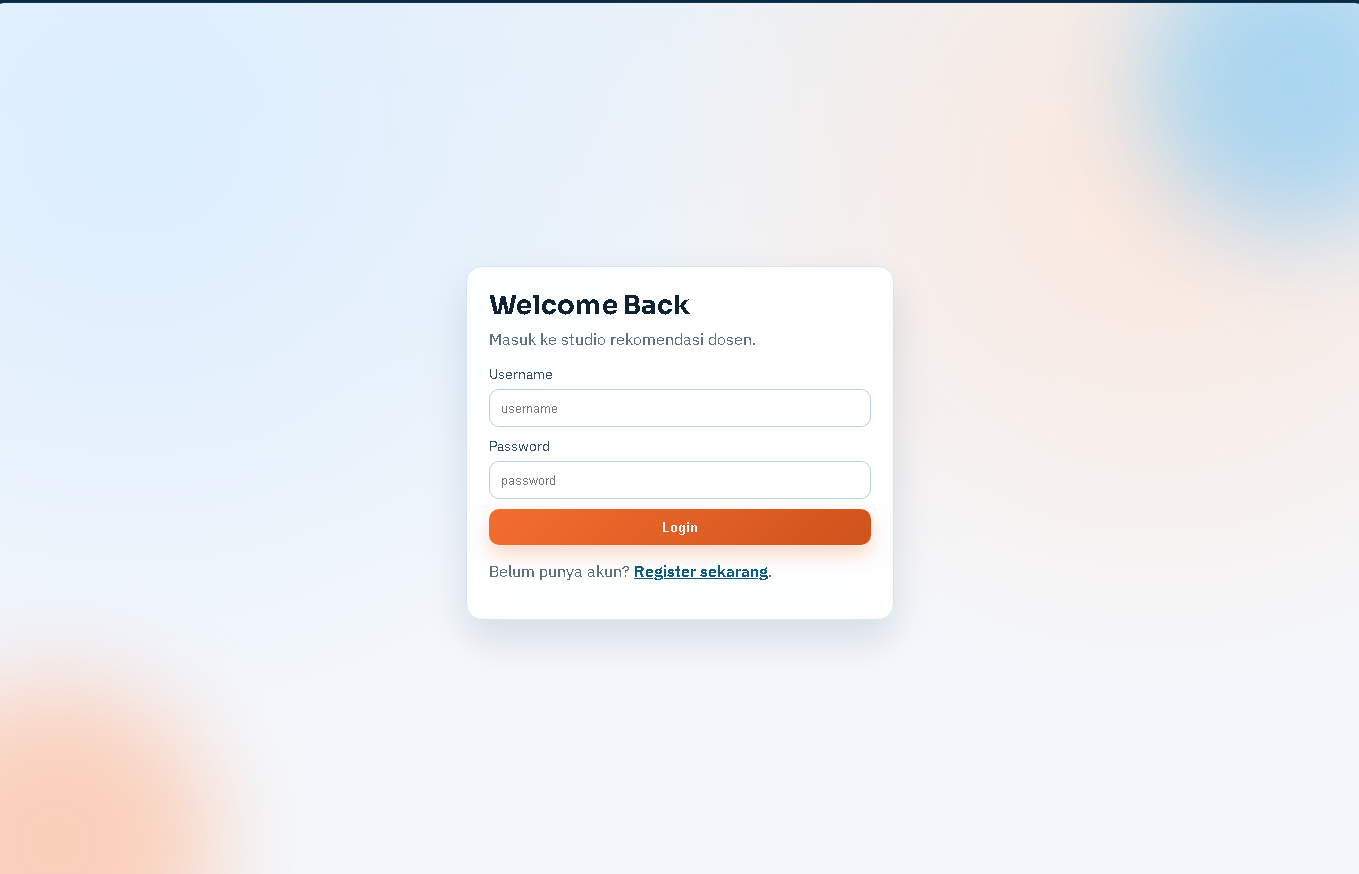
\includegraphics[width=0.7\linewidth]{pic/login.png}
    \end{center}
    \caption{Tampilan Halaman Login}
    \label{fig:login}
\end{figure}
        
Halaman login merupakan gerbang utama interaksi pengguna dengan sistem yang menyediakan formulir terstruktur untuk memasukkan data kredensial. Antarmuka (interface) ini mencakup kolom (field) username dan kata sandi yang telah didaftarkan oleh pengguna sebelumnya. Juga bila pengguna belum memiliki akun bisa mendaftarkan akun dengan memilih tombol registrasi. 

\subsubsection{Register Page}

\begin{figure}
    \begin{center}
        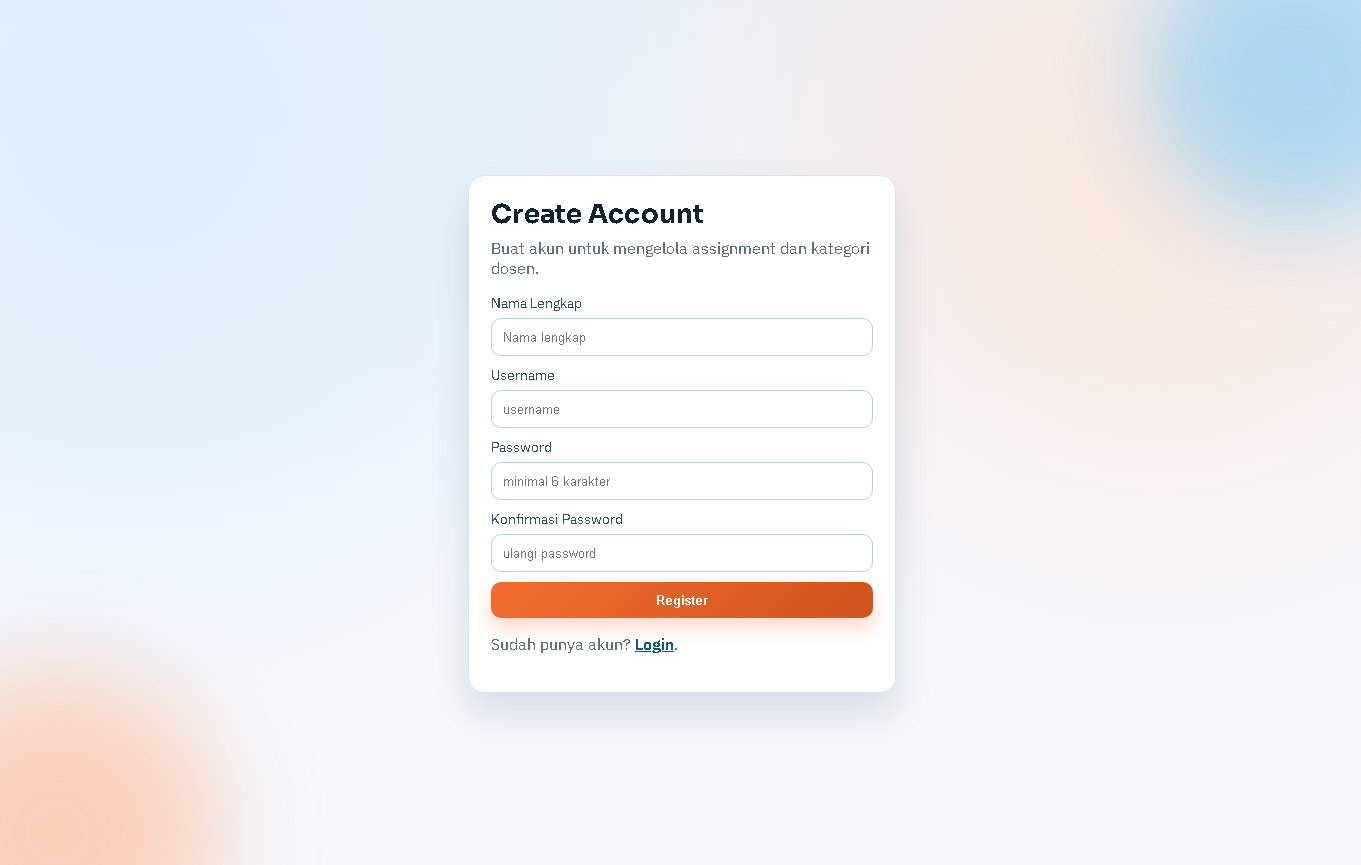
\includegraphics[width=0.7\linewidth]{pic/register.png}
    \end{center}
    \caption{Tampilan Halaman Register}
    \label{fig:register}
\end{figure}
        
Pada halaman ini pengguna dapat membuat akun dengan mengisi beberapa fields seperti nama lengkap, username, password dan konfirmasi password. Lalu proses dilanjutkan dengan memilih tombol registrasi setelah mengisi data dan akun akan otomatis dibuat. 

\subsubsection{Dashboard}

\begin{figure}
    \begin{center}
        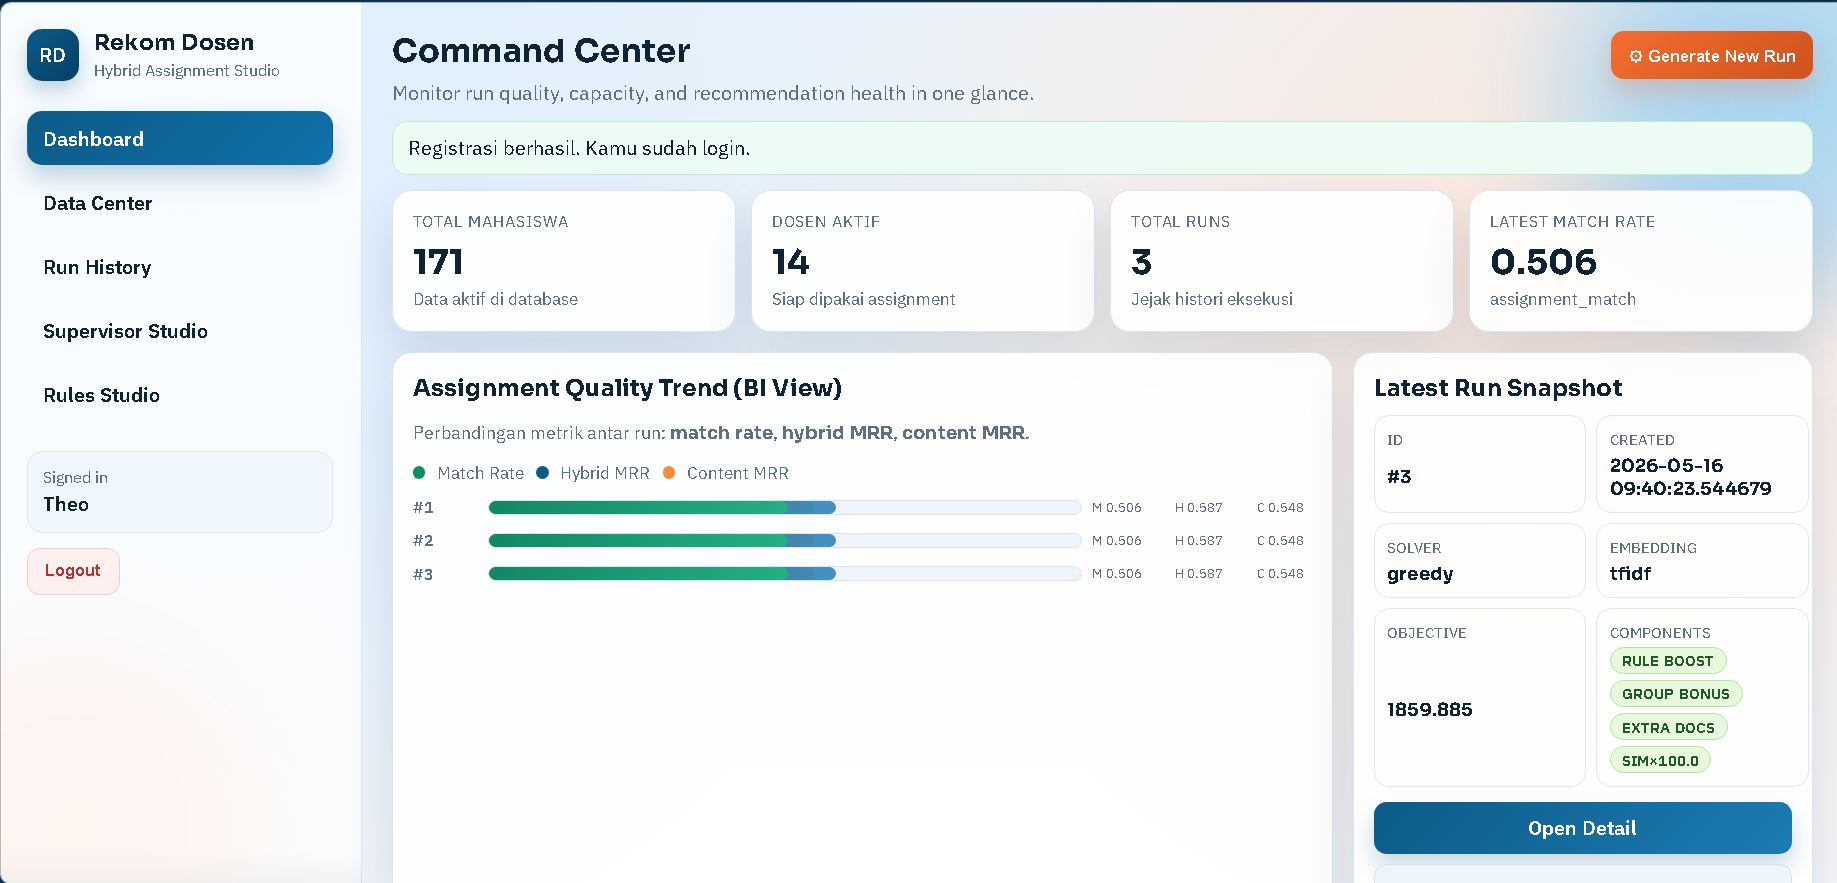
\includegraphics[width=0.7\linewidth]{pic/dashboard.png}
    \end{center}
    \caption{Tampilan Halaman Dashboard}
    \label{fig:dashboard}
\end{figure}
        
Halaman dashboard menyajikan ringkasan data statistik utama, meliputi total mahasiswa dan dosen yang telah terdaftar di dalam sistem. Selain itu, pengguna dapat memantau akumulasi proses eksekusi (total runs), tingkat akurasi pada eksekusi terakhir, serta rincian hasil evaluasi yang telah diproses. Fitur pada halaman ini juga memungkinkan pengguna untuk mengakses rincian run, dan inspect row, hingga melakukan ekspor data ke format Excel berdasarkan hasil eksekusi terbaru.  
\subsubsection{Data Center}

\begin{figure}
    \begin{center}
        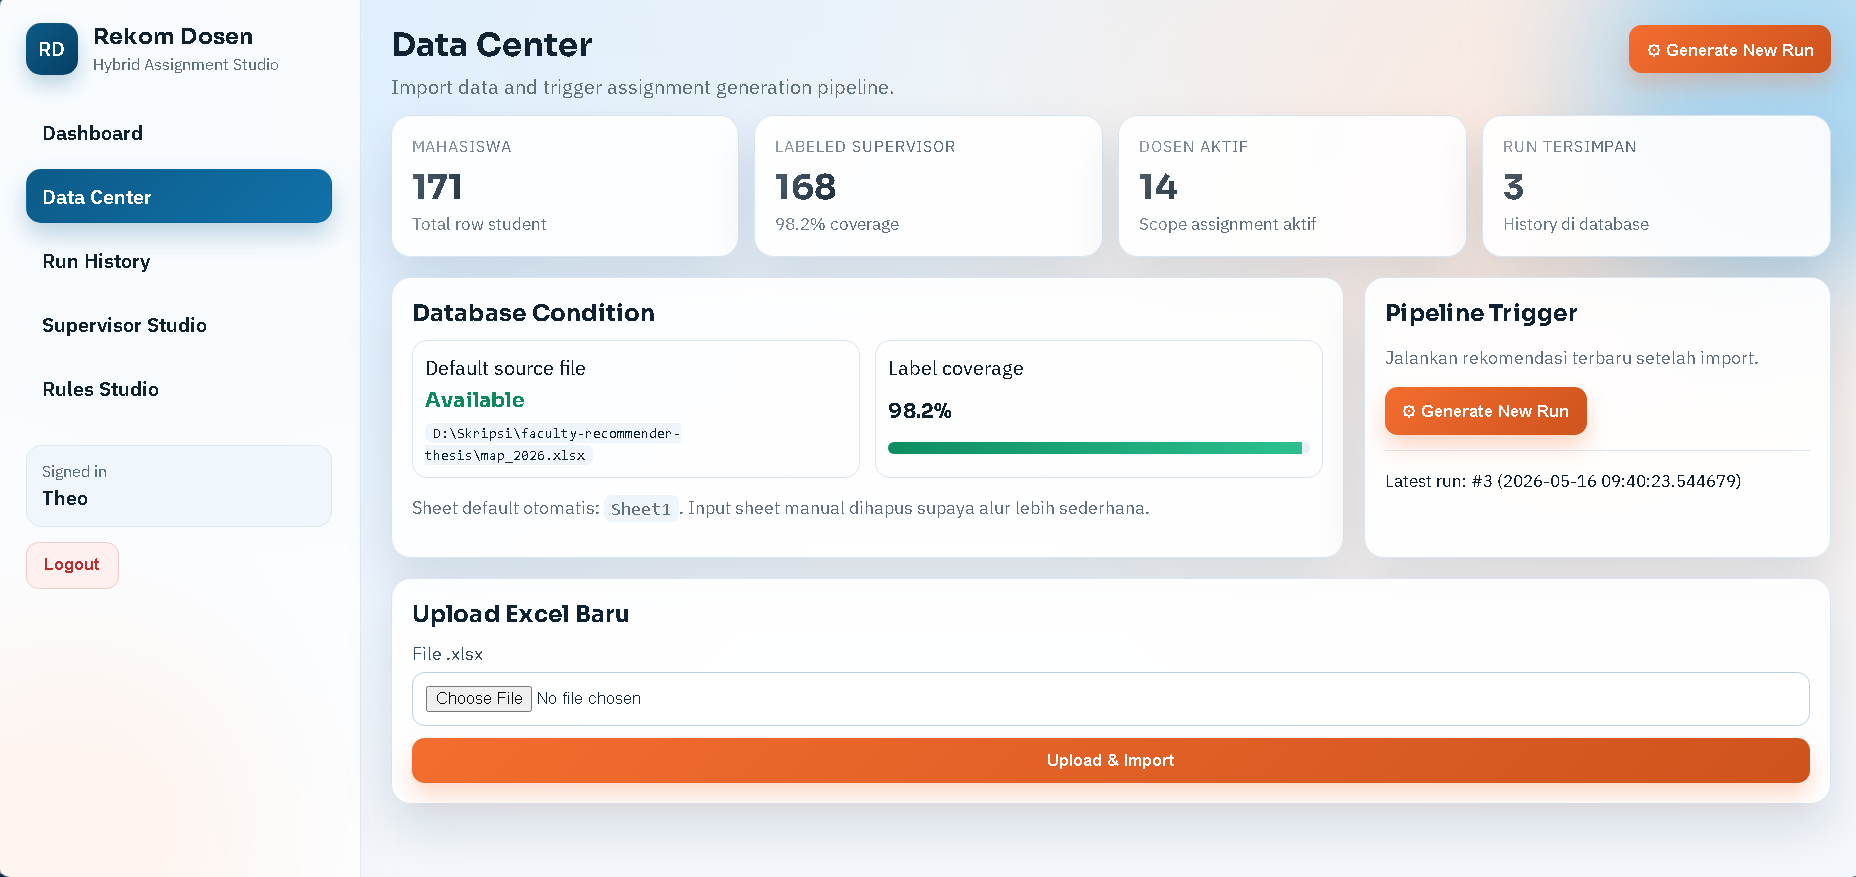
\includegraphics[width=0.7\linewidth]{pic/datacenter.png}
    \end{center}
    \caption{Tampilan Halaman Data Center}
    \label{fig:datacenter}
\end{figure}
        
Halaman ini berfungsi sebagai pusat pengelolaan data masukan (dataset) serta pengendali eksekusi awal (pipeline trigger) sistem. Peran utamanya adalah melakukan proses ETL (Extract, Transform, Load) guna memastikan kesiapan data mahasiswa dan dosen pembimbing sebelum diproses oleh algoritma rekomendasi. 

\subsubsection{Run History}

\begin{figure}
    \begin{center}
        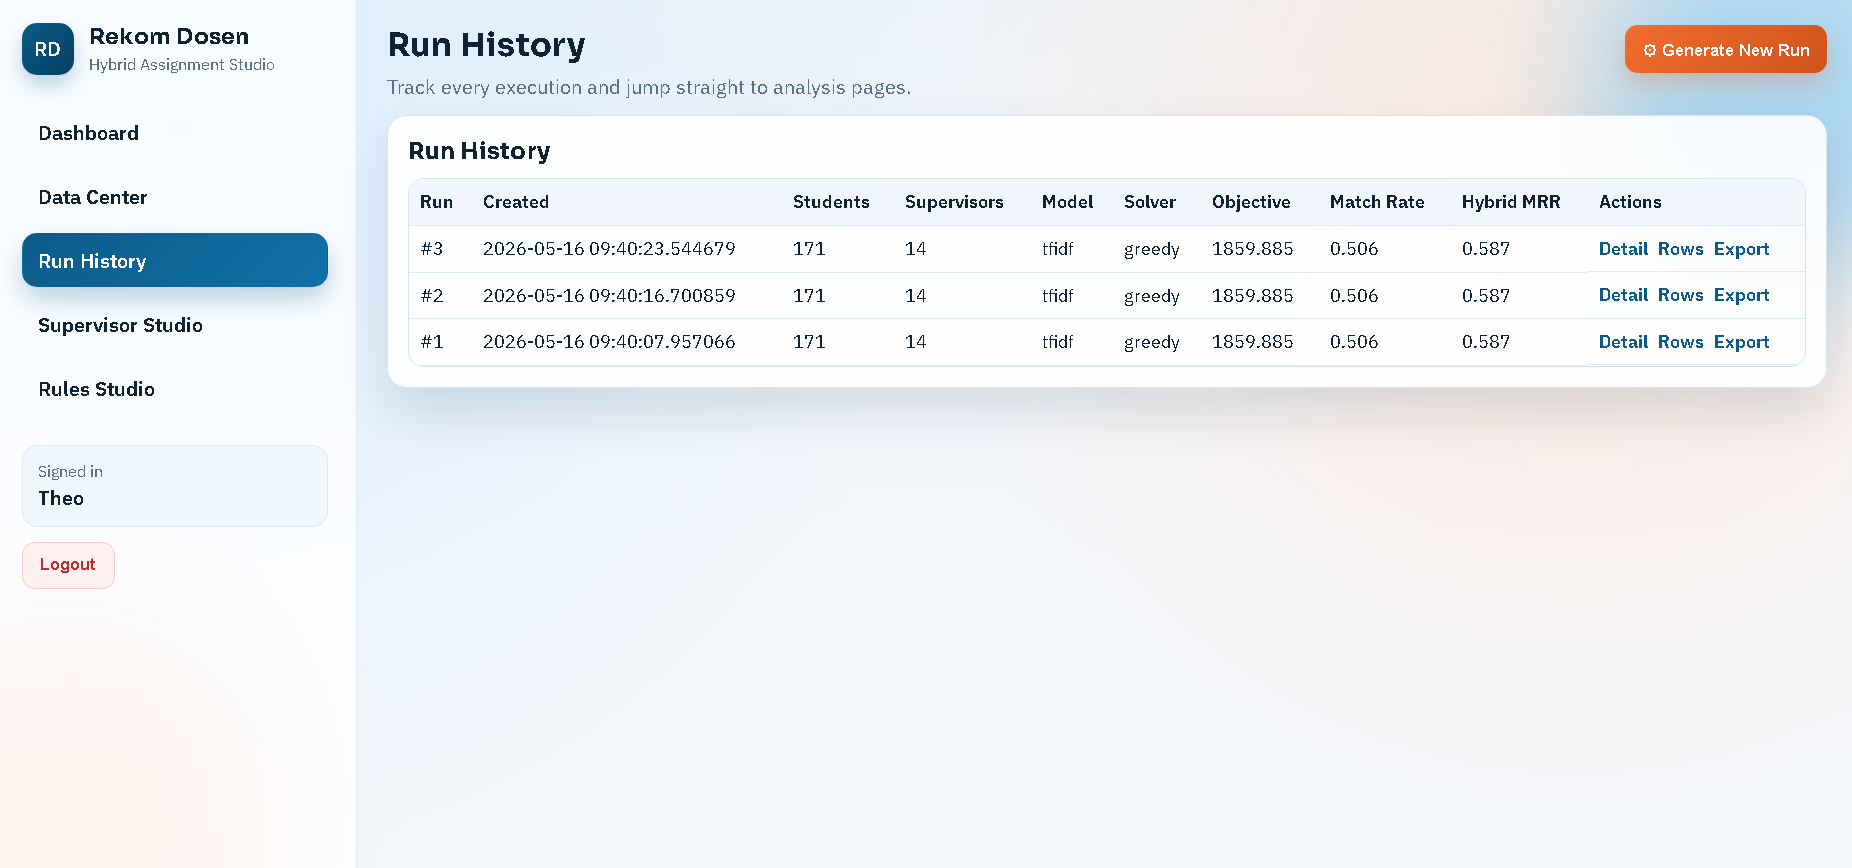
\includegraphics[width=0.7\linewidth]{pic/runhistory.png}
    \end{center}
    \caption{Tampilan Halaman Run History}
    \label{fig:runhistory}
\end{figure}
        
Halaman Run History menyajikan riwayat seluruh proses eksekusi run yang telah dilakukan oleh sistem. Informasi yang ditampilkan mencakup waktu eksekusi, jumlah mahasiswa dan dosen yang terlibat, model yang digunakan, serta hasil evaluasinya. Selain itu, pengguna dapat melakukan aksi lanjutan untuk meninjau rincian eksekusi detail run maupun mengekspor data ke dalam format Excel.   

\subsubsection{Run Details}

\begin{figure}
    \begin{center}
        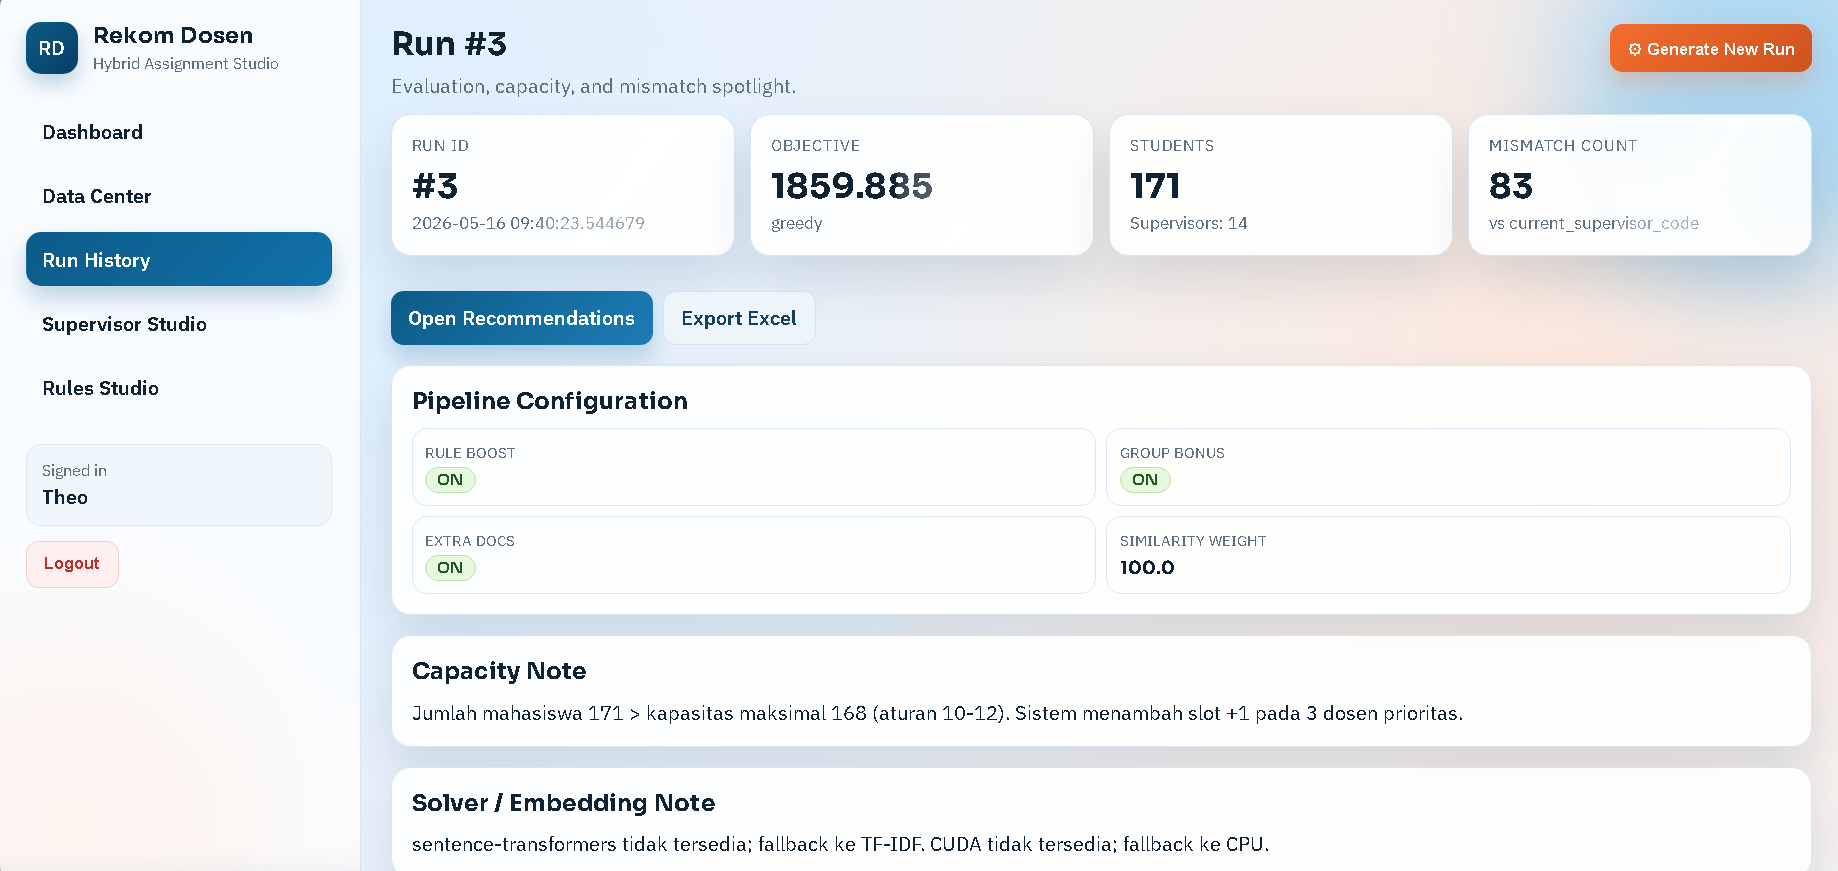
\includegraphics[width=0.7\linewidth]{pic/rundetails.png}
    \end{center}
    \caption{Tampilan Halaman Run Details}
    \label{fig:rundetails}
\end{figure}
        
Halaman Run Details menampilkan rincian hasil dari proses eksekusi run yang telah dilakukan. Informasi yang disajikan mencakup data spesifik untuk setiap mahasiswa, meliputi NIM, Nama, Track, Partner, Topik, Current Supervisor, Recommended Supervisor, Final Score, dan Rule Match. Selain itu, pengguna dapat menggunakan fitur filter untuk mempermudah pencarian data berdasarkan parameter tertentu, seperti nama, topik, maupun dosen  supervisor tertentu. . 

\subsubsection{Supervisor Studio}

\begin{figure}
    \begin{center}
        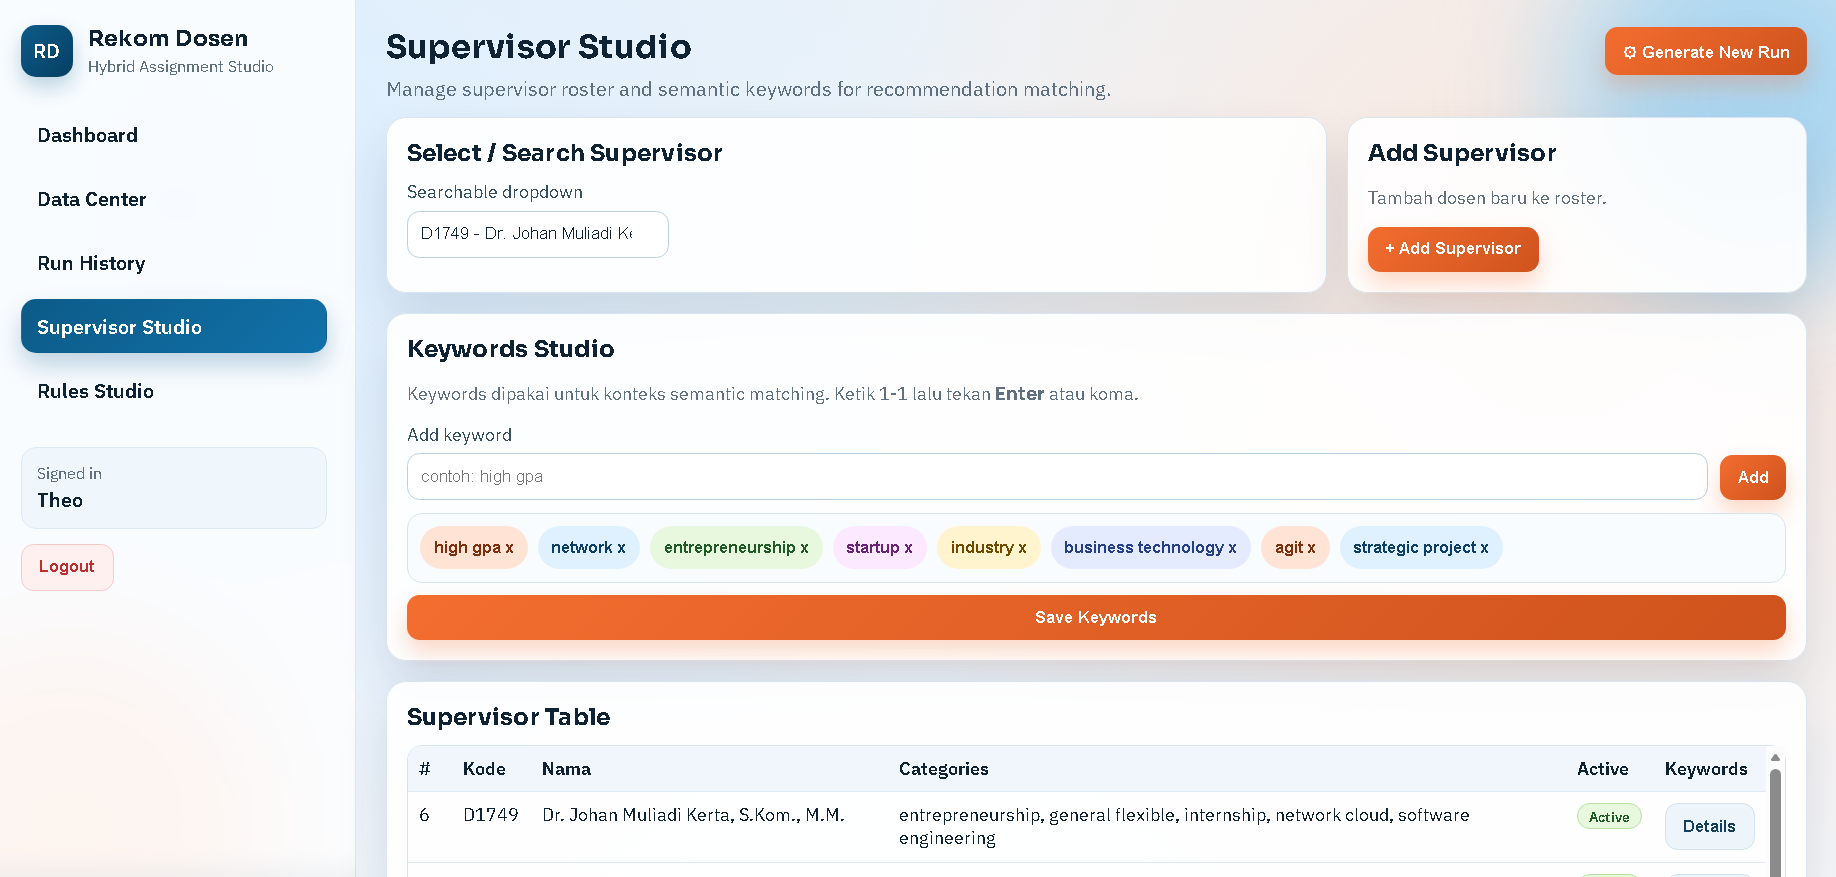
\includegraphics[width=0.7\linewidth]{pic/supervisorstudio.png}
    \end{center}
    \caption{Tampilan Halaman Supervisor Studio}
    \label{fig:supervisorstudio}
\end{figure}
        
Halaman Supervisor Studio berfungsi mengelola repositori dosen pembimbing dan semantic keywords. Fitur utama halaman ini meliputi searchable dropdown dan tombol Load Supervisor untuk pemanggilan profil dosen, serta Export Config Excel untuk pencadangan data. Selain itu, terdapat formulir Add Supervisor untuk perekaman data dosen baru, panel Keywords Studio untuk memanipulasi komponen chip kata kunci secara dinamis, dan Supervisor Table yang menyajikan akumulasi data dosen terdaftar secara terstruktur. 

\subsubsection{Rules Studio}

\begin{figure}
    \begin{center}
        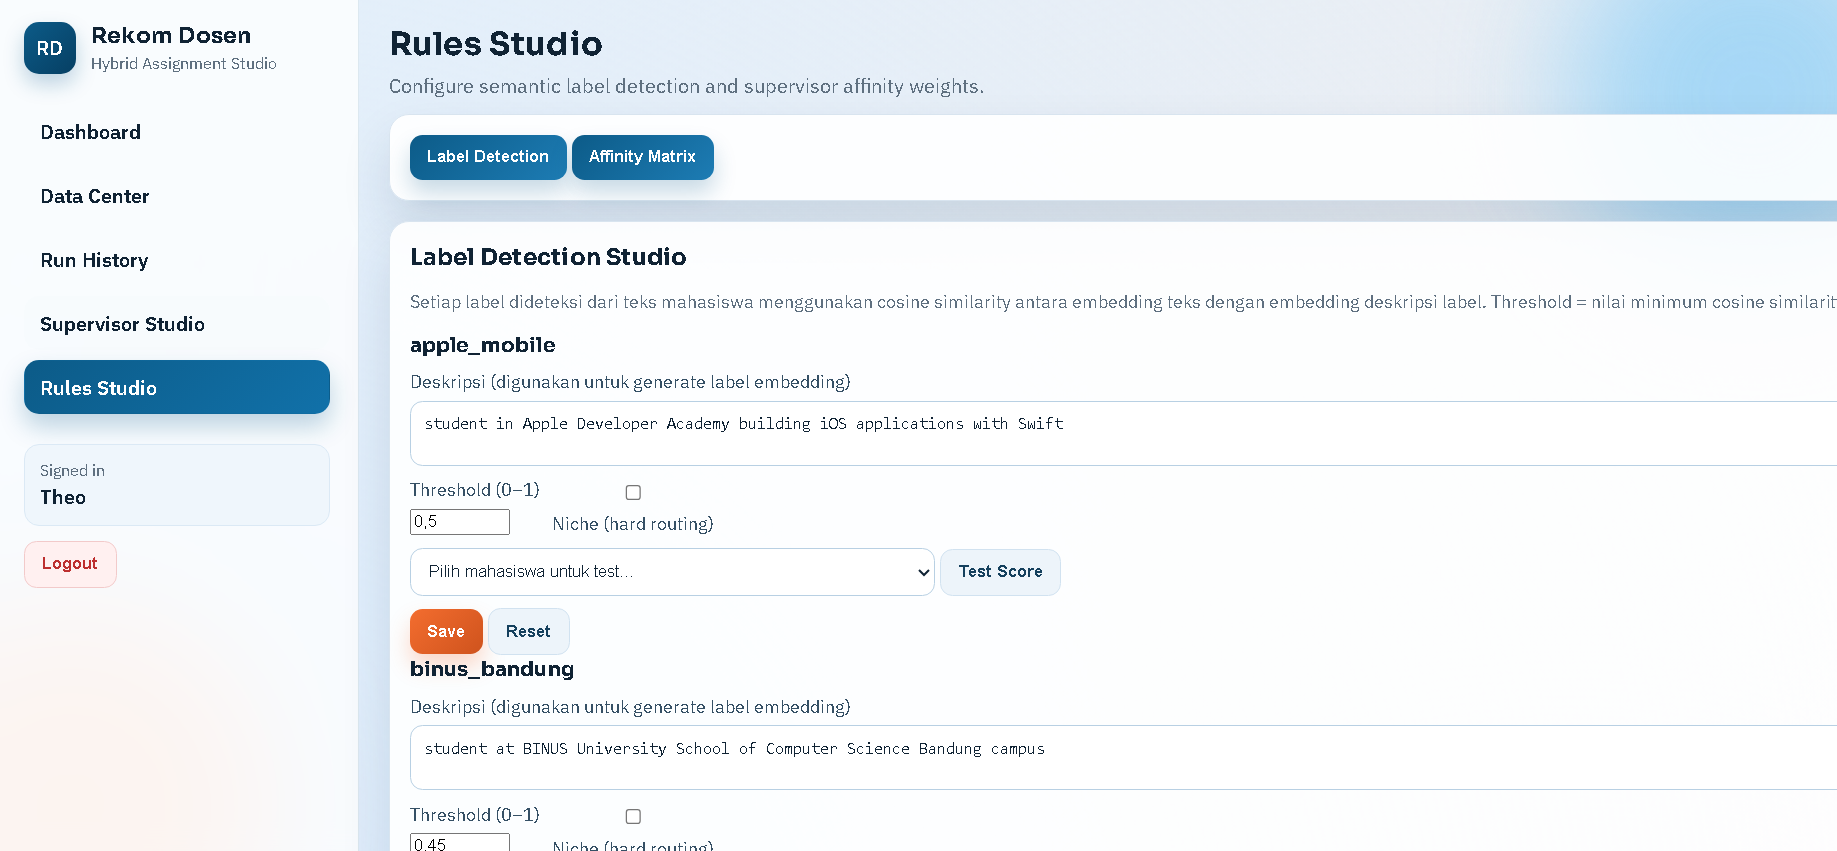
\includegraphics[width=0.7\linewidth]{pic/rulestudio.png}
    \end{center}
    \caption{Tampilan Halaman Rules Studio}
    \label{fig:rulestudio}
\end{figure}

Halaman Rules Studio berfungsi mengonfigurasi parameter klasifikasi label semantik yang digunakan dalam proses rekomendasi. Fitur utama meliputi pengaturan \textit{cosine similarity threshold} per label semantik, pengelolaan deskripsi label yang menentukan pemetaan profil mahasiswa ke kategori penugasan tertentu (seperti \texttt{apple\_mobile} atau \texttt{binus\_bandung}), serta pratinjau skor label untuk profil mahasiswa tertentu. Perubahan konfigurasi pada halaman ini akan berpengaruh pada proses deteksi label pada \textit{pipeline} run berikutnya.

\section{Evaluasi}

Pengujian Black Box dilakukan untuk memvalidasi fungsionalitas sistem dari sudut pandang pengguna tanpa melihat struktur kode internal. Fokus pengujian ini adalah memastikan bahwa setiap input memberikan output yang sesuai dengan spesifikasi kebutuhan sistem. Metode yang digunakan adalah Equivalence Partitioning, di mana data uji dibagi ke dalam beberapa kategori untuk menguji perilaku sistem terhadap input yang valid dan tidak valid. 

\subsection{Login Page}

Pada halaman ini terdapat tombol “Login” yang akan mengarahkan pengguna jika mengisi kredensial dengan benar. 

\begin{table}
 \centering
\begin{tabular}{|>{\fontsize{11}{14}\selectfont}p{0.5cm}|>{\fontsize{11}{14}\selectfont}p{4cm}|>{\fontsize{11}{14}\selectfont}p{3cm}|>{\fontsize{11}{14}\selectfont}p{4cm}|>{\fontsize{11}{14}\selectfont}p{1cm}|}
    \hline
\textbf{No} & \textbf{Skenario Pengujian} & \textbf{Data Uji} & \textbf{Hasil yang Diharapkan} & \textbf{Status }\\
    \hline
    1 & Login dengan kredensial valid  & Email dan kata sandi benar & Sistem mengarahkan pengguna ke dashboard & Pass  \\ 
    \hline
    2 & Login dengan kata sandi salah   & Email benar, kata sandi salah  & Sistem menampilkan message “Kredential Salah” & Pass  \\ 
    \hline
    3 & Login dengan email salah   &Email salah, kata sandi benar  &Sistem menampilkan message “Kredential Salah”  & Pass  \\ 
    \hline
\end{tabular}
\renewcommand{\arraystretch}{1}
	\caption{Skenario Login Page}
	\label{table:tab4.3.1}
\end{table}

\subsection{Register Page}

Pada halaman ini pengguna dapat membuat akun dengan mengisi data email dan password sebagai kredensial.

\begin{table}
 \centering
\begin{tabular}{|>{\fontsize{11}{14}\selectfont}p{0.5cm}|>{\fontsize{11}{14}\selectfont}p{4cm}|>{\fontsize{11}{14}\selectfont}p{3cm}|>{\fontsize{11}{14}\selectfont}p{4cm}|>{\fontsize{11}{14}\selectfont}p{1cm}|}
    \hline
\textbf{No} & \textbf{Skenario Pengujian} & \textbf{Data Uji} & \textbf{Hasil yang Diharapkan} & \textbf{Status }\\
    \hline
    1 & Mendaftarkan akun dengan email dan password   & Email dan kata sandi benar & Sistem menyimpan data email dan password pengguna & Pass  \\ 
    \hline
   2 & Mendaftarkan akun dengan kata sandi salah    & Email benar, kata sandi salah  & Sistem menampilkan message “Data tidak sesuai” & Pass  \\ 
    \hline
    3 & Mendaftarkan akun email salah    &Email salah, kata sandi benar  &Sistem menampilkan message “Data tidak sesuai”  & Pass  \\ 
    \hline
\end{tabular}
\renewcommand{\arraystretch}{1}
	\caption{Skenario Register Page}
	\label{table:tab4.4}
\end{table}

\subsection{Dashboard}

Pada halaman ini bertujuan pada fungsionalitas visual dan interaksi pada halaman Dashboard. Pengujian mencakup validasi tampilan data statistik, grafik tren, detail eksekusi terbaru, dan kontrol navigasi.

\begin{table}
 \centering
\begin{tabular}{|>{\fontsize{11}{14}\selectfont}p{0.5cm}|>{\fontsize{11}{14}\selectfont}p{4cm}|>{\fontsize{11}{14}\selectfont}p{3cm}|>{\fontsize{11}{14}\selectfont}p{4cm}|>{\fontsize{11}{14}\selectfont}p{1cm}|}
    \hline
\textbf{No} & \textbf{Skenario Pengujian} & \textbf{Data Uji} & \textbf{Hasil yang Diharapkan} & \textbf{Status }\\
    \hline
    1 & Klik Menu "Dashboard"   & - & Sistem mengarahkan pengguna ke halaman Data Center  & Pass  \\ 
    \hline
   2 & Klik menu “Run History”  & -  & Sistem mengarahkan pengguna ke halaman Run History  & Pass  \\ 
    \hline
    3 &Klik menu “Supervisor Studio”     & -  & Sistem mengarahkan pengguna ke halaman Supervisor Studio   & Pass  \\ 
    \hline
     4 &Klik menu “Rules Studio”      & -  & Sistem mengarahkan pengguna ke halaman Rules Studio    & Pass  \\ 
    \hline
     5 & Klik tombol “Generate New Run”      & -  & Sistem akan mengarahkan pengguna ke tampilan untuk melakukan run baru    & Pass  \\ 
    \hline
     6 & Klik tombol “Open Detail”      & -  & Sistem mengarahkan pengguna ke halaman detail dari run terakhir   & Pass  \\ 
    \hline
     7 & Klik tombol “Inspect Rows”       & -  & Sistem akan mengarahkan pengguna melihat data pada Run History   & Pass  \\ 
    \hline
     8 & Klik tombol “Export Excel”      & -  & Sistem akan melakukan export pada data run terakhir.    & Pass  \\ 
    \hline
    9 & Sistem menampilkan data pada Summary Cards       & -  & Data yang ditampilkan sesuai dengan database   & Pass  \\ 
    \hline
    10 & Sistem menampikan data pada Quality Trend      & -  & Sistem menampikan tooltop detail nilai Match Rate, Hybrid MRR, dan Content MRR    & Pass  \\ 
    \hline
    11 & Sistem menampikan Informasi Snapshot      & -  & Sistem menampilkan data dari run paling baru     & Pass  \\ 
    \hline
\end{tabular}
\renewcommand{\arraystretch}{1}
	\caption{Skenario Dashboard}
	\label{table:tab4.5}
\end{table}

\subsection{Data Center}

Pada halaman ini pengujian bertujuan untuk memvalidasi fungsi manajemen  import data serta interaksi pipeline trigger. Halaman ini krusial karena bertindak sebagai penyedia data utama sebelum sistem menjalankan algoritma rekomendasi. 

\begin{table}
 \centering
\begin{tabular}{|>{\fontsize{11}{14}\selectfont}p{0.5cm}|>{\fontsize{11}{14}\selectfont}p{4cm}|>{\fontsize{11}{14}\selectfont}p{3cm}|>{\fontsize{11}{14}\selectfont}p{4cm}|>{\fontsize{11}{14}\selectfont}p{1cm}|}
    \hline
\textbf{No} & \textbf{Skenario Pengujian} & \textbf{Data Uji} & \textbf{Hasil yang Diharapkan} & \textbf{Status }\\
    \hline
    1 & Upload Data Kosong   & - & Sistem menolak proses import dan menampikan error message  & Pass  \\ 
    \hline
   2 & Upload Data dengan Format Salah  & -  & Sistem menolak proses import dan menampilkan  error message   & Pass  \\ 
    \hline
    3 & Upload Valid     & -  & File berhasil disimpan, dan sistem akan menampilkan data pada sumarry cards.    & Pass  \\ 
    \hline
     4 & Data pada Summary Cards sesuai      & -  & Data yang ditampilkan sesuai dengan data upload     & Pass  \\ 
    \hline
     5 & Klik tombol “Generate New Run”      & -  & Sistem akan mengarahkan pengguna ke tampilan untuk melakukan run baru    & Pass  \\ 
    \hline
    
\end{tabular}
\renewcommand{\arraystretch}{1}
	\caption{Skenario Data Center}
	\label{table:tab4.6}
\end{table}

\subsection{Generate New Run}

Pada halaman ini pengujian berfungsi untuk melalukan pengecekan ketika pengguna ingin melakukan run baru dengan memilih model dan rules boost yang akan diterapkan pada run tersebut. 

\begin{table}
 \centering
\begin{tabular}{|>{\fontsize{11}{14}\selectfont}p{0.5cm}|>{\fontsize{11}{14}\selectfont}p{4cm}|>{\fontsize{11}{14}\selectfont}p{3cm}|>{\fontsize{11}{14}\selectfont}p{4cm}|>{\fontsize{11}{14}\selectfont}p{1cm}|}
    \hline
\textbf{No} & \textbf{Skenario Pengujian} & \textbf{Data Uji} & \textbf{Hasil yang Diharapkan} & \textbf{Status }\\
    \hline
    1 & Memilih Model   & - & Model yang dipilih akan terlihat dengan ditandai berwarna oren  & Pass  \\ 
    \hline
   2 & Mengaktifkan Group Bonus  & -  & Toggle group bonus yang dipilih akan berubah warna menjadi oren   & Pass  \\
    \hline
    3 & Menonaktifkan Group Bonus     & -  & Toggle group bonus kembali ke kondisi nonaktif  & Pass  \\ 
    \hline
     4 & Cancel Run     & -  & Sistem akan menutup pop-up new run  \\ 
    \hline
     5 & Eksekusi Run Baru     & -  & Sistem akan menjalankan rekomendasi dengan model dan rules yang dipilih    & Pass  \\ 
    \hline
    
\end{tabular}
\renewcommand{\arraystretch}{1}
	\caption{Skenario Generate New Run}
	\label{table:tab4.7}
\end{table}

\subsection{Run History}

Pada halaman ini  bertujuan untuk memastikan sistem mampu menyajikan daftar riwayat  run algoritma secara kronologis dan akurat. Fokus utama meliputi kebenaran metadata yang ditampilkan serta fungsionalitas button. 

\begin{table}
 \centering
\begin{tabular}{|>{\fontsize{11}{14}\selectfont}p{0.5cm}|>{\fontsize{11}{14}\selectfont}p{4cm}|>{\fontsize{11}{14}\selectfont}p{3cm}|>{\fontsize{11}{14}\selectfont}p{4cm}|>{\fontsize{11}{14}\selectfont}p{1cm}|}
    \hline
\textbf{No} & \textbf{Skenario Pengujian} & \textbf{Data Uji} & \textbf{Hasil yang Diharapkan} & \textbf{Status }\\
    \hline
    1 & Sistem menampikan tabel riwayat run yang sudah dijalankan  & - & Sistem menampilkan kolom Run ID, Created, Students, Supervisor, Model, Solver, Objective, Match Rate, dan Hybrid MRR   & Pass  \\ 
    \hline
   2 & Tabel Riwayat di Tampilkan Berdasarkan Urutan Terakhir Dijalankan  & -  & Data ditampilkan secara urut (Descending)    & Pass  \\ 
    \hline
    3 & Klik tombol “Details Row” pada salah satu ID Run      & -  & Sistem berpindah ke halaman detail page dari run yang dipilih     & Pass  \\ 
    \hline
     4 & Klik tombol “Export Data’ pada salah satu ID Run      & -  & Sistem melakukan export data sesuai ID Run yang dipilih    & Pass  \\ 
    \hline
     5 & Klik tombol “ Generate New Run pada page Run History       & -  & Sistem mengarahkan pengguna ke halaman pembuatan run baru     & Pass  \\ 
    \hline
    
\end{tabular}
\renewcommand{\arraystretch}{1}
	\caption{Skenario Run History}
	\label{table:tab4.8}
\end{table}

\subsection{Supervisor Studio}

Pada halaman ini bertujuan untuk memastikan sistem memvalidasi fitur pengelolaan data dosen pembimbing beserta kata kunci semantik.

\begin{table}
 \centering
\begin{tabular}{|>{\fontsize{11}{14}\selectfont}p{0.5cm}|>{\fontsize{11}{14}\selectfont}p{4cm}|>{\fontsize{11}{14}\selectfont}p{3cm}|>{\fontsize{11}{14}\selectfont}p{4cm}|>{\fontsize{11}{14}\selectfont}p{1cm}|}
    \hline
\textbf{No} & \textbf{Skenario Pengujian} & \textbf{Data Uji} & \textbf{Hasil yang Diharapkan} & \textbf{Status }\\
    \hline
    1 & Membuka menu dropdown dan mencari berdasarkan nama atau kode dosen   & - & Sistem menyaring data secara dinamis berdasarkan data dosen yang dicari    & Pass  \\ 
    \hline
   2 & Memilih salah satu nama dosen kemudian menekan tombol “Load Supervisor”   & -  & Sistem menampilkan profil dosen dan keyword yang sesuai dengan dosen tersebut     & Pass  \\ 
    \hline
    3 & Menekan tombol “Export Config”       & -  & Sistem akan mengunduh berkas excel berisikan data dosen dan profilnya.      & Pass  \\ 
    \hline
     4 & Mengetikkan keyword baru pada kolom “Add Keyword”    & -  & Keyword di daftarkan di dalam daftar keyword     & Pass  \\ 
    \hline
     5 & Menekan tombol (X) pada salah satu komponen chip       & -  & Chip keyword akan dihapuskan       & Pass  \\ 
    \hline
     6 & Menekan tombol “Save Keywords” setelah melakukan perubahan chip       & -  & Sistem memperbarui daftar keyword semantik pada dosen di database        & Pass  \\ 
    \hline
    
\end{tabular}
\renewcommand{\arraystretch}{1}
	\caption{Skenario Supervisor Studio}
	\label{table:tab4.9}
\end{table}


\subsection{Rules Studio}

Pada halaman ini testing bertujuan untuk memvalidasi fleksibilitas pengaturan rules. Halaman ini mengontrol cosine similarity threshold dan deskripsi label semantik yang menentukan bagaimana profil minat mahasiswa dipetakan ke dalam kategori penugasan tertentu (seperti apple\_mobile atau binus\_bandung).  

\begin{table}
 \centering
\begin{tabular}{|>{\fontsize{11}{14}\selectfont}p{0.5cm}|>{\fontsize{11}{14}\selectfont}p{4cm}|>{\fontsize{11}{14}\selectfont}p{3cm}|>{\fontsize{11}{14}\selectfont}p{4cm}|>{\fontsize{11}{14}\selectfont}p{1cm}|}
    \hline
\textbf{No} & \textbf{Skenario Pengujian} & \textbf{Data Uji} & \textbf{Hasil yang Diharapkan} & \textbf{Status }\\
    \hline
    1 & Membuka menu dropdown dan mencari berdasarkan nama atau kode dosen   & - & Sistem menyaring data secara dinamis berdasarkan data dosen yang dicari    & Pass  \\ 
    \hline
   2 & Memilih salah satu nama dosen kemudian menekan tombol “Load Supervisor”   & -  & Sistem menampilkan profil dosen dan keyword yang sesuai dengan dosen tersebut     & Pass  \\ 
    \hline
    3 & Menekan tombol “Export Config”       & -  & Sistem akan mengunduh berkas excel berisikan data dosen dan profilnya.      & Pass  \\ 
    \hline
     4 & Mengetikkan keyword baru pada kolom “Add Keyword”    & -  & Keyword di daftarkan di dalam daftar keyword     & Pass  \\ 
    \hline
     5 & Menekan tombol (X) pada salah satu komponen chip       & -  & Chip keyword akan dihapuskan       & Pass  \\ 
    \hline
     6 & Menekan tombol “Save Keywords” setelah melakukan perubahan chip       & -  & Sistem memperbarui daftar keyword semantik pada dosen di database        & Pass  \\ 
    \hline
    
\end{tabular}
\renewcommand{\arraystretch}{1}
	\caption{Skenario Supervisor Studio}
	\label{table:tab4.10}
\end{table}